\section{Introduction}

\begin{figure}
    \centering
    \begin{subfigure}[b]{\columnwidth}
        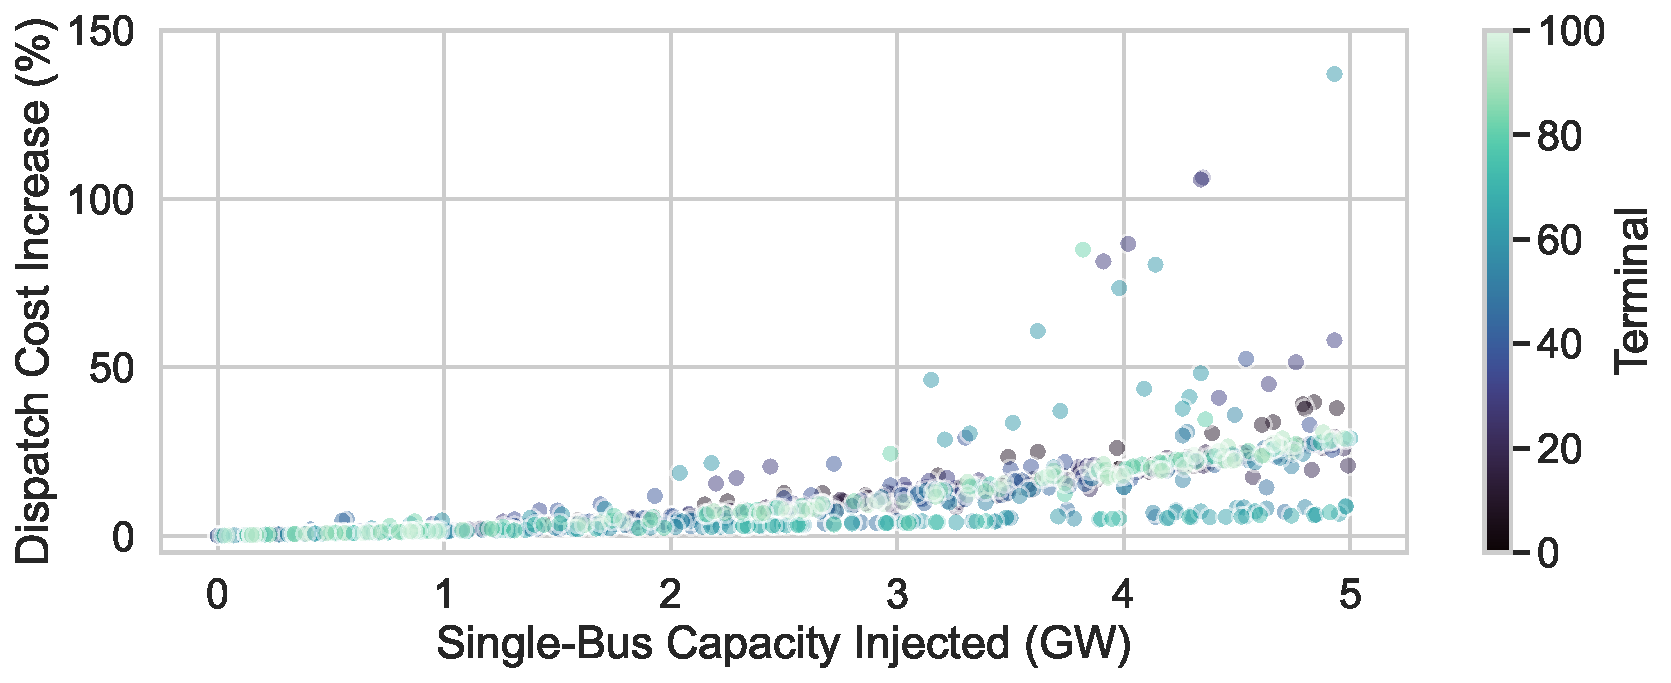
\includegraphics[width=\linewidth]{figures/dispatch_cost_percent_increase.pdf}
        \caption{Dispatch cost increase.}
        \label{fig:dispatch-cost-cloud}
    \end{subfigure}
    \begin{subfigure}[b]{\columnwidth}
        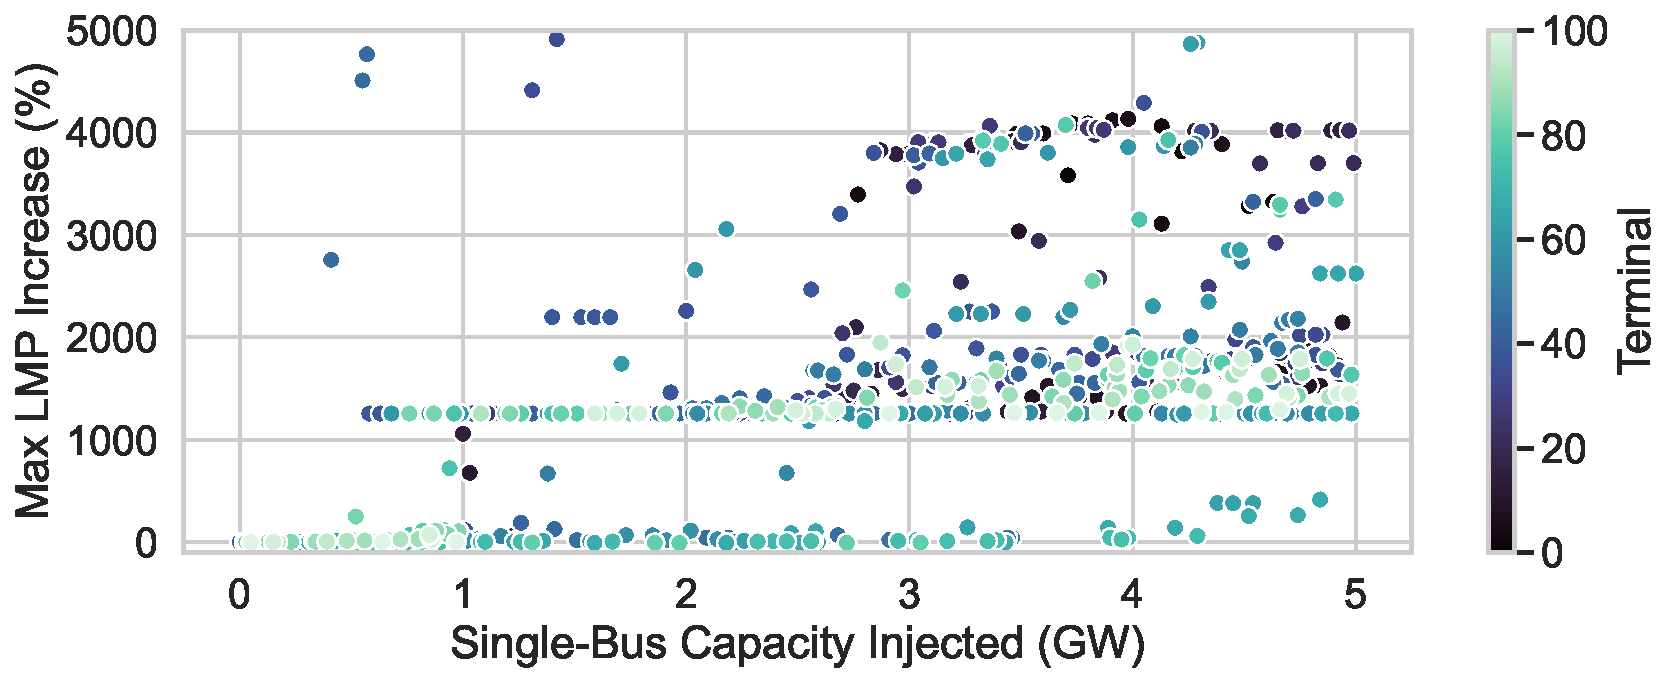
\includegraphics[width=\linewidth]{figures/max_lmp_increase.pdf}
        \caption{Max locational marginal price (LMP).}
        \label{fig:max-lmp-cloud}
    \end{subfigure}
    \caption{Dispatch and locational marginal price (LMP) for WECC when provisioning a data center load at a single terminal. We notice that in general, the cost of operating the system and LMP rises with increasing capacity.}
    \label{fig:cloud-plots}
\end{figure}

\textbf{Motivation.} The rapid expansion of AI computing infrastructure has led to requests for electric load connection at an unprecedented rate. 
Individual data-center campuses are now proposed at
hundreds of megawatts to gigawatt scale~\cite{stargate, gw-scale}, with interconnection requests arriving
on compressed timelines and often concentrated at a small number of transmission buses~\cite{EPRI2024PoweringDataCenters, dukerethinking}. As a result, the planning question facing system operators and regulators is no longer only whether sufficient generation exists to serve new demand, but \emph{where} large loads should be connected and how concentrated those connections should be across the network.

Public concerns around large datacenter interconnections often center around sustainability~\cite{},
rate hikes~\cite{}, and downstream cost impacts for other consumers~\cite{}. These effects arise through known
mechanisms. Changes in congestion and dispatch induced by large-load siting decisions 
are seen in the system as higher locational marginal prices (LMPs) and total 
dispatch costs. When a new load activates transmission constraints, system operators 
must redispatch generation away from least-cost units toward more expensive marginal 
resources. This raises systemwide dispatch costs and increases LMPs at constrained 
locations, with effects that can extend well beyond the bus where the load was added. 
LMPs are not prices paid by the consumer, but instead signs that point towards 
potentially higher rates. Large load owners, such as data-center operators, are 
exposed directly through nodal energy prices and congestion charges. Other consumers may be affected indirectly via congestion cost allocation or rate increases that recover higher system operating costs over time. 


While these effects are well
studied in economic planning, existing work has not been used to compare 
alternative load placement strategies for the same aggregate demand. As data-center 
demand scales from tens of megawatts to multiple gigawatts, this limitation becomes 
more pronounced.

A central challenge our work demonstrates is that a grid's response to new load is highly nonlinear. Adding capacity at some
locations can be absorbed with modest impact on the system at large, while similar additions elsewhere can
trigger congestion and price escalation once specific transmission constraints or critical lines bind. These ``knee''
points are location-dependent and are not visible in traditional peak/off-peak screening studies. 
As one can see in Figure~\ref{fig:cloud-plots} both LMPs and dispatch cost increase 
system-wide no matter where a datacenter is placed. For LMPs in Figure~\ref{fig:max-lmp-cloud}, 
some nodes do exist in the bottom right regime with a low change in price with added 
capacity, yet the vast majority of nodes see a massive increase in LMP.


In this study, we develop a framework for stress-testing large datacenter load siting
decisions. Rather than proposing a single optimal placement, we evaluate how alternative allocations of
a fixed interconnection capacity across candidate buses affect system dispatch cost, LMP distributions,
and congestion patterns under operation. We explicitly distinguish provisioned utility-side interconnect capacity from normalized temporal load profiles, enabling apples-to-apples
comparison across different capacity concentrations and site counts. The framework emphasizes
diagnostics, such as changes in the set of binding transmission constraints, to explain why
distribution helps in some regimes and fails in others.

We apply the framework to a 101-bus representation of the U.S. Western Interconnection and study
large-load injections ranging from tens of megawatts to multiple gigawatts. Our results reveal....

Our contributions are as follows.
\begin{enumerate}
    \item We produce a comparative framework for evaluating large-load siting strategies that quantifies congestion, dispatch-cost, and LMP impacts.
    \item We demonstrate that distributing large loads across multiple nodes can mitigate LMP spikes as compared to single site injection.
    \item We explore how distribution of load with other grid levers such as transmission upgrades and extra storage can improve the amount of deployable capacity.
    \item We compare our proposed optimization framework to that of naive baselines demonstrating that we are able to offset the pricing and congestion effects through distributed placement.
    \item We quantify the ways in which workload differences and different site load profiles can lead to regret and optimality gap's in placed data centers.
\end{enumerate}
